%-------------------------------------------------------------------------------
\section{Data Disguises}
\label{sec:disguises}
%-------------------------------------------------------------------------------
\begin{figure}[t!]
    \centering
    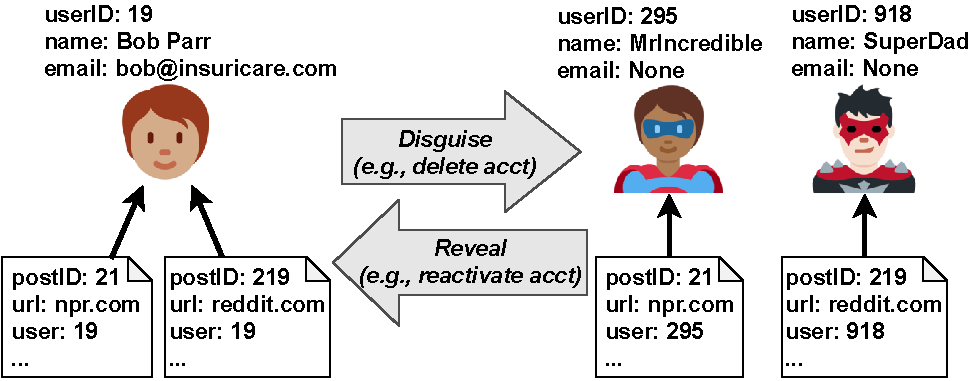
\includegraphics[width=0.5\textwidth]{img/disguises}

    \caption{Disguises move the target object (in this example, a user Bob) from an identity-revealing
    guise to privacy-preserving guises. \lyt{TODO need to change from reveal?}}
    \label{fig:example}
\end{figure}

%\lyt{TODO (Frans): drive w/explicit example of table rows and foreign key relationships, too
%abstract. Start with Figure~\ref{fig:arch}?}

\begin{figure*}[t!]
    \centering
    \footnotesize
\begin{tabular}{@{}c|c|c|c@{}}
\textbf{User Transformation Spec} & \textbf{User Object} & \textbf{Guise 1} &
    \textbf{Guise 2} \\
\begin{lstlisting}[language=Rust]
"id":       IDAttribute,
"name":     Gen(Random),
"active":   Gen(Default(false)),
"darkmode": CopyAll,
"notifs":   CopyOnce+Gen(Default(false)),
"tag_id":   GenForeignKey,
\end{lstlisting}
    &
\begin{lstlisting}[language=Rust]
"id":       19,
"name":     BobParr,
"active":   true,
"darkmode": false,
"notifs":   true,
"tag_id":   11
\end{lstlisting}
&
\begin{lstlisting}[language=Rust]
"id":       295,
"name":     MrIncredible,
"active":   false,
"darkmode": false,
"notifs":   true,
"tag_id":   81483
\end{lstlisting}
&
\begin{lstlisting}[language=Rust]
"id":       918,
"name":     SuperDad,
"active":   false,
"darkmode": false,
"notifs":   false,
"tag_id":   15592
\end{lstlisting}
\end{tabular}
    \caption{Creating two guises of an example user (of a synthetic application schema).}
    \label{fig:guises}
\end{figure*}

%
The key idea behind \emph{data disguising} is to associate multiple \emph{guises} with a target data
object (\ie a row in a relational database). Guises vary in how they reveal identities or preserve privacy.
%
Objects move between different guises by means of disguises---a set of constrained privacy
transformations.

Figure~\ref{fig:example} illustrates this with the example of user account deletion.
%
When his account is active, user Bob's profile is associated with his true identity and all his
contributions to the site (an identity-revealing guise).
%
When Bob deletes his account, his profile and contributions move to different, privacy-preserving
guises: his name has been anonymized, his email address has been redacted, and his contributions
have been decorrelated and attributed to individual, unidentified user guises.
%

At any given moment, an application's data object graph comprises a mix of identity-revealing guises
and privacy-preserving ones. Disguises split and combine individual guises when triggered.

%
The application developer writes a disguise for each privacy transformation needed
in the application.
%
%This specification is a declarative statement similar to a relational schema, with entries for
%graph vertices (objects) to be transformed.
%and directed edges (relationships between pairs of objects)
%to be transformed (see \S\ref{sec:spec}).
%
We assume that:
\begin{enumerate}[nosep]
  \item developers use their domain knowledge to write correct and complete disguises;
    %\lyt{a bit worried about ``complete'' here}
  \item application code handles the different guises appropriately (\eg in
    displaying them); and
  \item different guises of the same object have the same structure (\eg they can be
    rows in the same table).
\end{enumerate}
%
A data disguising tool takes the disguise specification and turns it into storage operations that
apply the transformation.
% (disguise) or its reverse (reveal).

%
%\lyt{Not sure if we need this paragraph anymore.}
%Data disguising builds on the existing structure of web applications.
%
%Web applications are often structured as object graphs, either explicitly~\cite{tao, delf},
%through an object-relational model (ORM)~\cite{orm}, or implicitly via foreign keys (edges)
%between tables (vertices) in relational databases.
%
%Data disguises transform this object graph.

\subsection{Writing Disguises}
Disguises offer developers the ability to transform objects into guises: they can modify
guises at per-attribute (\ie per-column) granularity, or \emph{decorrelate} an object from any guise that
references it (via \eg foreign-key relationships). Decorrelation creates multiple guises for the
object, reassociating each referencing object to a unique guise to preserve referential integrity.
Objects can also be removed entirely.
Developers must specify both the desired transformations, and a predicate for each transformation
that selects the objects to be transformed.
\lyt{This predicate is specified as a read-only SQL WHERE clause}.

To create a guise from an object, developers specify how to transform attributes of the
object (\eg table column values) into guise attributes.
%
Figure~\ref{fig:guises} shows an example, producing guises for user objects.
%
User objects have identifier \texttt{id}; a reference \texttt{tag\_id}
associates the user via a foreign key constraint to tag objects.
%

%
Guises always have unique, random identifiers.
%
Developers choose how to create other guise attributes, selecting from among the following:
%
\paragraph{(1) Copy object content.}
%
Guises of the same object all share the object's attribute values.
%
If the attribute is a reference attribute (\eg a foreign key column), all guises will refer to the same object.
%
%
Copying allows developers to retain the object's content, without worrying about how to
synthesize attribute values for guises.
%
%However, this should only be chosen if guise attribute
%values cannot be generated, or if this attribute says little about the true identity of the
%entity.
For example, in Figure~\ref{fig:guises} the \texttt{darkmode} attribute is copied in
all guises.
%; the \texttt{darkmode} attribute reveals very little about the underlying user's
%identity.

\paragraph{(2) Generate new content.}
%
To create new attributes, developers specify whether the guise's value should be random,
a default value, or generated from the object's attribute value via a custom function (\eg hashing 
the value).
%
Figure~\ref{fig:guises} illustrates an example of random (\texttt{name}) and default
(\texttt{active}) generated value attributes.
%
%
Creating new guise reference attributes (\eg new foreign key relationships) requires
creating a new guise for the referenced object in order to maintain referential
integrity;
the data disguise rewrites the reference to point to the new guise.
%
In Figure~\ref{fig:guises}, creating two user guises requires creating two
tag guises, and the tag guises' identifiers become the user guises' foreign keys.
%

\paragraph{(3) Copy object content, but only once.}
%
One guise copies the attribute value from the object, but all other guises generate new
values (as described above).
%
\texttt{notifs} in Figure~\ref{fig:guises} illustrates how the attribute is copied once.
%
This enables the application to retain the original object semantics (\eg a count of how many
users want notifications) without creating duplicates.
%


